加载了网络之后,~Cytoscape~的界面如图~\ref{fig:2.1}~所示。

\begin{figure}[!h]
\centering
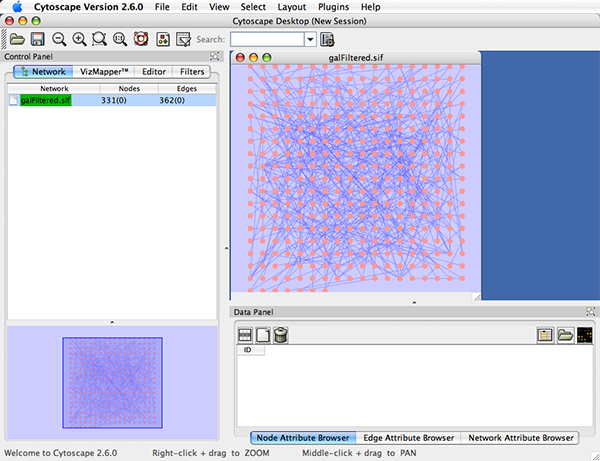
\includegraphics[width=\textwidth]{images/cytoscape_startup_network_26.png}
\caption{~Cytoscape~加载网络后的界面截图}
\label{fig:2.1}
\end{figure}

主界面由多个组件构成,包括:
\begin{itemize}
\item 顶部的菜单(稍后会对各个菜单做详细介绍)。
\item 工具栏,包含了各种常用功能。从菜单中也能使用这些功能。鼠标指针在这些图标上停留片刻就能看到有关的提示。
\item 网络管理面板(左上方的面板)。其中有可关闭的网络全局浏览面板(左下方)。
\item 网络查看主窗口,网络就显示在这个窗口中。
\item 属性浏览器面板(底部的面板),显示所选择的节点和边的属性。在这个面板中还可以对这些属性的值进行修改。
\end{itemize}

网络管理和属性浏览器面板是可以拖拽的标签面板,被称为~CytoPanels~。通过点击~CytoPanel~右上角的浮动窗口(Float Window)控件~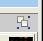
\includegraphics{images/float_icon.png}~可以将这些面板设为浮动状态。

如果选择了这个控件,例如属性浏览器面板上的这个控件,就会出现两个~Cytoscape~的窗口,一个是主窗口,另一个是名为CytoPanel 2的新窗口,如下图所示。当鼠标指针指向单元格时,会看到弹出信息。

{\centering
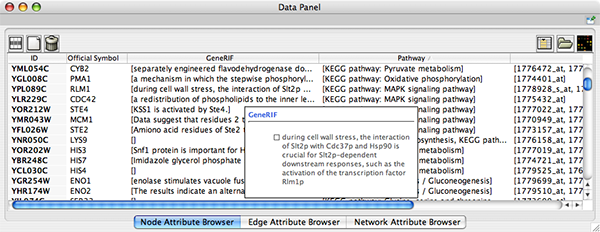
\includegraphics[width=\textwidth]{images/attribute_browser_26.png}
}

在图中可以看到,CytoPanel 2~现在有一个~Dock Window~控件。如果点选这个控件,这个窗口就会回到主窗口中。

Cytoscape~还提供了一个用于构建和编辑网络的编辑器,把面板中的节点和边拖拽到主网络视图窗口中就能创建和编辑网络。用Visual Style可以定义节点的形状以及边的箭头。只需要选择CytoPanel 1中的Editor标签就能编辑网络。下图展示了一个编辑器,Visual Style是BioMoleculeEditor。

{\centering
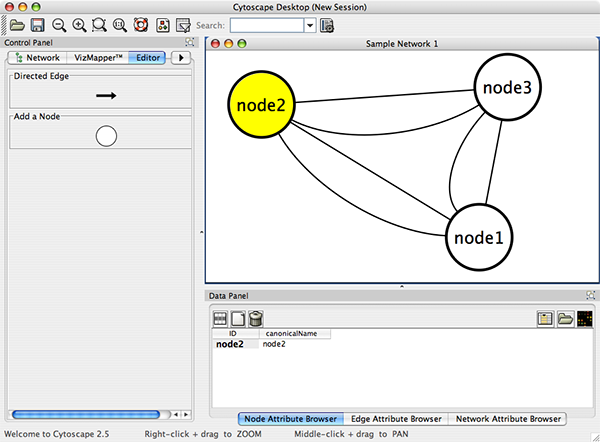
\includegraphics[width=\textwidth]{images/editor_25.png}}

\section{菜单}
	\subsection{File}
	File菜单中含有最基本的文件操作功能:File $\rightarrow$ Open~用于打开~Cytoscape~
	会话文件;File $\rightarrow$ New~用于新建空白网络,也可以从现用的网络创建新网络;
	File $\rightarrow$ Save~用于保存会话文件;File $\rightarrow$ Import~用于导入网
	络或属性数据;File $\rightarrow$ Export~用于导出数据和图片。File $\rightarrow$ 
	Print用于打印,File $\rightarrow$ Quit~则是关闭所有的~Cytoscape~窗口,并推出程
	序。

	\begin{figure}[!h]
	\centerline{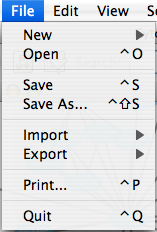
\includegraphics[scale=0.6]{images/menu_file_26.png} }
	\end{figure}

	\subsection{Edit}
	Edit菜单中提供了用于属性浏览器、网络编辑器和布局的撤销(Undo)和重做(Redo)功能。
	
	还有创建和销毁视图(网络的显示方法)和网络(网络的原始数据,并不可视化的)的菜单项,以及用于从当前网络中删除所选节点和边的菜单项。通过 Edit $\rightarrow$ Undo~可以恢复被删除的节点和边。配置和插件的设置可以通过Edit $\rightarrow$ Preferences $\rightarrow$ Properties来编辑。

	\begin{figure}[!h]
	\centerline{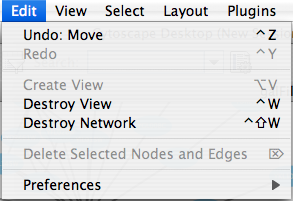
\includegraphics[scale=0.6]{images/menu_edit_26.png}}
	\end{figure}

	\subsection{View}
在~View~菜单中可以控制网络管理面板(CytoPanel 1)、属性浏览器(CytoPanel 2)、网络概览(在CytoPanel
1中)和VizMapper的显示和隐藏。

	\begin{figure}[!h]
	\centerline{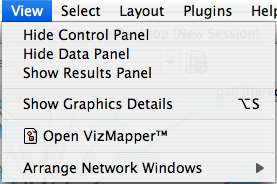
\includegraphics[scale=0.6]{images/menu_view_26.png}}
	\end{figure}

	\subsection{Select}
	在~Select~菜单中含有选择节点和边的各种选项。还有Select $\rightarrow$ Use Filter选项,用于根据节点或边的某些属性创建自动的过滤器。

	\begin{figure}[!h]
	\centerline{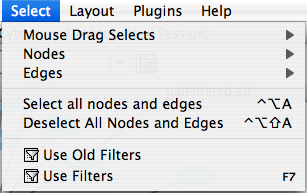
\includegraphics[scale=0.6]{images/menu_select_26.png}}
	\end{figure}

	\subsection{Layout}
	通过~Layout~菜单可以控制网络显示的形式。该菜单上半部分(Rotate,Scale,Align and
	 Distribute)是用于控制网络的显示。菜单的下半部分是用于自动布局网络的各种布局算法。

	\begin{figure}[!h]
	\centerline{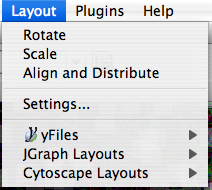
\includegraphics[scale=0.6]{images/menu_layout_25.png}}
	\end{figure}
	
		
	
	\subsection{Plugins}
	Plugins~菜单中提供了插件管理功能(安装、升级和删除),以及插件所添加的选项,比如
	~Agilent Literature Search~或~Merge Networks~。具体的内容取决于所加载的插件。
	\footnote{注意:在~\href{http://cytoscape.org/plugins2.php}
	{http://cytoscape.org/plugins2.php}~上有Cytoscape~插件的介绍。}
	
	\begin{figure}[!h]
	\centerline{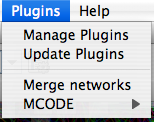
\includegraphics[scale=0.6]{images/menu_plugins_25.png}}
	\end{figure}
	
	\subsection{Help}
	在Help菜单中可以打开在线帮助,浏览本手册内容。“About...”则会显示正在运行的~Cytos
	cape~的版本信息。
	\begin{figure}[!h]
	\centerline{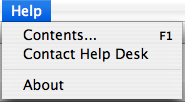
\includegraphics[scale=0.6]{images/menu_help_25.png}}
	\end{figure}

\section{网络管理}
	Cytoscape~2.3之后的版本都可以同时加载多个网络,有无视图都可以。网络中存放着用户
	加载所有节点和边,以及用户做指定的视图。同一个网络可以有多个视图。网络(以及相应
	的视图)可以有序地组织在一起。

    下图中展示了多个网络同时加载,并按层次结构组织的例子:

    \begin{figure}[!h]
    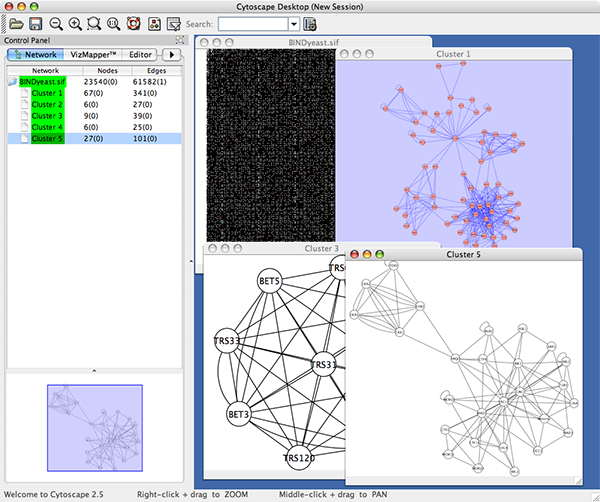
\includegraphics[width=\textwidth]{images/cytoscape_network_hierarchy_25.png}
    \end{figure}

    网络管理器(CytoPanel 1右上方的树状显示窗口)展示了当前所加载的网络。点击其中的
    网络就会在主窗口里面显示该网络的视图。在网络管理器中会显示各个网络的名称和尺寸(
    节点和边的数量)。如果网络是从文件中加载的,网络的名称就是文件名。
    
    对于那些规模较大的网络(数千个点和边),需要较长的时间才能显示出来。正因为如此, 
    Cytoscape中的网络可以不包含“视图”(View)。带有视图的网络以绿色高亮显示,而没有
    视图的网络则以红色高亮显示。在网络管理器中网络的名称上点击鼠标右键,就能创建或是
    销毁视图,通过Edit菜单也能实现同样的操作。用同样的方法可以销毁已加载的网络。在上
    图中,加载了七个网络,其中六个绿色的是有视图的,而红色的那个则是没有视图的 
    。\footnote{译者注:图中总共只有六个网络,都是绿色的,似乎原文有误。}

Cytoscape中的某些特定操作会创建出新的网络。如果新网络是从原有的网络中创建的,例如选择
原网络中的部分节点,将这些节点复制到新网络中(用File~$\to$~New~$\to$~Network option),
在这种情况下新网络就会显示为原网络的子网络。Cytoscape的这种显示方法使得用户能很快地
看出网络间的关系。上图中树顶部的那些网络就是这样生成的。

在网络视图窗口中,所有网络视图都会以窗口的形式显示出来。通过窗口右上角的窗口标准控件
可以最大化、最小化或是销毁网络视图。

    \subsection{网络窗口排列}

在同时处理多个网络时,可以用View$\to$Arrange Network Windows菜单项中的命令来重新排
布窗口的排列方式。

    \begin{figure}[!h]
    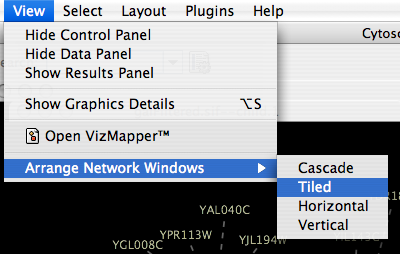
\includegraphics[width=.5\textwidth]{images/arrange_26_1.png} 
    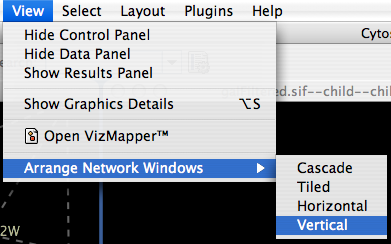
\includegraphics[width=.5\textwidth]{images/arrange_26_3.png}
    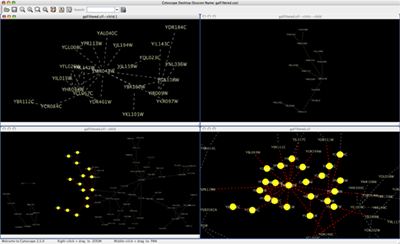
\includegraphics[width=.5\textwidth]{images/arrange_26_2.png}
    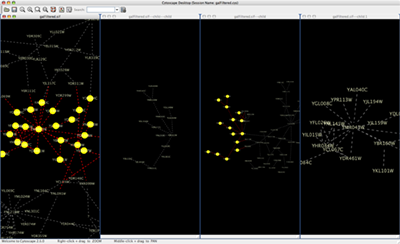
\includegraphics[width=.5\textwidth]{images/arrange_26_4.png}
    \end{figure}


\section{网络概览窗口}

网络概览窗口中会显示网络的概况(或者说是“鸟瞰”)。这样就能比较方便地浏览规模较大的网
络。蓝色矩形表示当前网络视图窗口中所显示的范围,用鼠标拖动这个矩形框就能浏览网络的其
他部分。放大或缩小网络时,矩形框的大小也会自动的做出相应的变化。
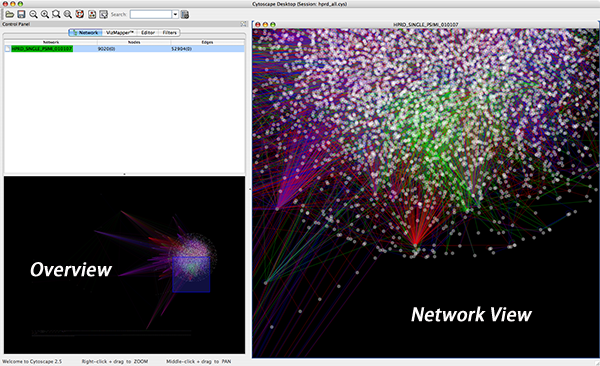
\includegraphics[width=\textwidth]{images/network_overview_25.png}
	




